\documentclass{paper}
%\usepackage{nomencl}
\usepackage{nomencl}
\usepackage{amsmath}
\usepackage{graphicx}
\usepackage{subfigure}
\usepackage{parskip}
%\usepackage{minted}
\usepackage[toc,page]{appendix}
\usepackage{csquotes}
\usepackage{framed}
\usepackage{amsthm}

\theoremstyle{theorem}
\newtheorem{theorem}{Theorem}[section]
 
\theoremstyle{definition}
\newtheorem{definition}{Definition}[section]

\theoremstyle{remark}
\newtheorem{remark}{Remark}[section]
%\usepackage{biblatex}
%\makenomenclature
\title{Motion Planning}
\author{A. Giavaras}
\date{}

\begin{document}
\maketitle
\tableofcontents

\clearpage
\section{Motion Planning}
\label{motion_planning}

Motion planning is the problem of finding a continuous collision free path from an initial
configuration (or state) to a goal. On board an autonomous vehicle, the capability to prevent
collisions also depends on the sensing and control. Critically, motion planning is a necessary
component for the safe operation of an autonomous vehicles. Apart from an efficient algorithm
for motion planning, one should also consider  the problem of embedding the motion planner 
into a software system in which all tasks are required to satisfy hard deadlines. 

We will discuss such a  framework that can be used as a basis for incorporating approximately complete motion planning algorithms within a
hard real-time system. This framework ensures that deadlines can be satisfied, with only mild
constraints on other software. Two motion planning algorithms are presented as a verification
of the framework, and are applied to solving dynamic motion planning problems related to the
safe and efficient navigation of autonomous systems.


\subsection{Introduction}
\label{introduction_motion_planning}
A challenging problem in the development of unmanned and autonomous systems is to develop
navigation strategies that are efficient, by minimising metrics such as transit time and power
usage, while also minimising the risk of collisions. This problem is subject to uncertainty
and partial information regarding the state of the vehicle, the obstacles, and the responses of
the vehicle to inputs. Robust strategies for safe and efficient navigation require replanning to
compensate for uncertainty and changes in the environment. The success of such strategies
is dependent on the quality of sensing, planning and control, and on the temporal interactions
between those tasks.


The consequences of failing to perform sensing, planning or control within a suitable dead-
line can result in failure to observe obstacles, produce safe paths or accurately track a path.
Consistent failure to meet deadlines can have serious effects including poor performance with
respect to mission objectives or loss of vehicle, such as when a collision occurs.

\subsection{Safe navigation}
Safe navigation depends on being able to plan paths or trajectories that prevent collisions with
obstacles. In the case of autonomous vehicles these obstacles can be either static, such as
terrain or buildings, or dynamic, such as other moving vehicles.

In cases where an environment contains only static obstacles the task of finding safe paths
can be addressed by solving a motion planning problem \cite{LaValle2006}. A plan produced in this way
is only safe if the environment is fully observable and does not change over time, a case which
does not occur except in highly structured workspaces.

\begin{framed}
\theoremstyle{remark}
\begin{remark}{\textbf{Fully Observable Environment}}
 
\end{remark}
\end{framed}

More realistic environments would include obstacles that move over time and obstacles
that must be detected using sensors. This more difficult task can be addressed by replanning
when the environment changes, a process known as \textbf{dynamic motion planning}.


Using an analogy from control theory, motion planning can be thought of as {\em open-loop},
while dynamic motion planning can be considered its {\em closed-loop} equivalent. This highlights that 
the replanning is used to minimise errors resulting from unforeseen environmental changes. 
Furthermore, it is also useful to consider the task of safe navigation as a cycle of sensing, planning
and control or actuation as shown in Figure \ref{sense_plan_control_tasks_cycle}.

\begin{figure}[!htb]
\begin{center}
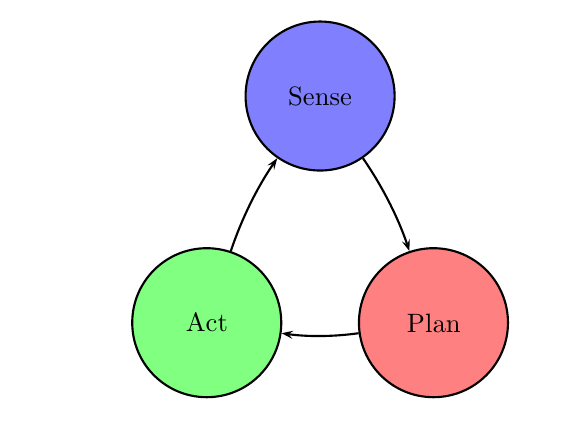
\includegraphics[scale=0.280]{img/motion_planning/sense_plan_control_tasks_cycle.jpeg}
\end{center}
\caption{ Sensing, planning and control tasks.}
\label{sense_plan_control_tasks_cycle}
\end{figure}

The sensing task is responsible for mapping and localization. Mapping involves measuring,
and in some cases predicting, locations of obstacles based on sensor observations. Localization
is the task of finding the configuration (location and pose) of the vehicle. The quality of
localization and mapping estimates is dependent on the types and properties of the sensors
used. A significant external factor which influences localization and mapping relates to how
quickly new observations are acquired, as compared to how quickly the vehicle moves.

The actuation task takes the sensed location of the vehicle and the path output of the mo-
tion planner, and produces inputs to the actuators. These inputs are chosen so as to minimise
path-tracking errors. The capability to track a path accurately depends on a number of factors
including: the magnitude of environmental disturbances, sensors, actuators and the implemen-
tation of the controller, including the rate at which the controller is updated at.

The planning process uses a single mapping and localization estimate to produce a collision
free path from the current configuration, to a goal configuration, determined based on the
current mission objective. While planning is being conducted, no new information can be
taken into account.

The capability to navigate safely depends on the quality of sensing, planning and control,
and the interaction between those tasks. Interactions between tasks include direct coupling
due to transfers of inputs and outputs, and indirect coupling that results from time taken for
each task to execute. Excessive delays by any task could result in a collision.


\subsubsection{Time critical planning}
\label{time_critical_planning}

The combination of minimal computational resources, high cost of failure through collision
and inter-coupling between the software tasks necessitate careful consideration of software
design alternatives on-board autonomous vehicles.

The need to support long-term missions with minimal human interaction imposes constraints on the design of autonomous systems. 
In particular, vehicle designers must find an
appropriate trade-off between \cite{Walker2011}

\begin{itemize}
\item Payload
\item Energy storage
\item Endurance
\item Sensing
\item Actuation
\item Computing capability
\end{itemize}

Constraints on computational resources tend to introduce trade-offs between performance
and other factors that tend to be less critical in traditional software design. For example,
an open issue in energy aware computing involves finding a suitable compromises between
the power consumption and speed required to execute a piece of software \cite{Walker2011}.
Similarly, safety critical software systems are required to produce results within a time limit or
risk catastrophic failure. With regard to planning for autonomous vehicles, failure to identify
new plans within an acceptable time limit can potentially result in a collision. For this
reason the hard real-time aspect of the computing constraints becomes crucial.

\begin{framed}
\theoremstyle{remark}
\begin{remark}{\textbf{Temporal Inter-Coupling}}
 
The temporal inter-coupling which occurs between sensing, planning and actuation is a
phenomenon that is frequently ignored in planning literature. The rare examples in which
the problem is considered [BV02, HKLR02], make the assumptions that minor collisions are
acceptable. In this work, the cost of a collision of an autonomous system makes such an
assumption unacceptable.
\end{remark}
\end{framed}


\begin{framed}
\theoremstyle{remark}
\begin{remark}{\textbf{Anytime Algorithms}}
 
Perhaps the best known results for planning under time constraints are those based on any-
time algorithms [BD89]. These algorithms progressively refine an initial solution, improving
quality as time permits. Such an approach is less applicable in cases like motion planning subject 
to kinematic and dynamic constraints, where finding an initial solution is time consuming.
\end{remark}
\end{framed}


Work on real-world autonomous systems is targeted towards deployment in complex, unstructured, 
time-variant and partially observable environments. The need to achieve safe navigation in these types of environments 
necessitates the use of dynamic motion planning algorithms.
Safe operation of an autonomous system requires that critical tasks (sensing, planning and
control), execute in a timely manner. Failure to do this can lead to errors in localization (vehicle
state), mapping (obstacle state and geometries), path tracking, and most importantly for this
work, path generation. Sufficiently large errors in any of these areas can result in degradation
in mission performance, or in the worst case, failure due to collisions \cite{Walker2011}.



\subsection{Motion planning}

Safe and efficient navigation is a task of significant interest in robotics, and particularly
mobile robotics. It involves finding a continuous path that can be followed from an initial
configuration (or state) to a goal configuration. A safe path is one that prevents collisions with
obstacles, and an efficient path is one which minimises cost. In real-world environments, safe
navigation depends on sensing, motion planning and control.

Safe and efficient navigation is a task of significant interest in robotics, and particularly
mobile robotics. It involves finding a continuous path that can be followed from an initial
configuration (or state) to a goal configuration. A safe path is one that prevents collisions with
obstacles, and an efficient path is one which minimises cost. In real-world environments, safe
navigation depends on sensing, motion planning and control.
One of the challenges of safe navigation relates to the quantity and reliability of informa-
tion available about the environment. Put simply, if there are inaccuracies in the estimated
location of the vehicle or obstacles, then there is risk that a collision will occur. To ensure that
an accurate model of the environment is available, vehicles are equipped with sensors capa-
ble of measuring the workspace around the vehicle. Sensor observations are used to identify
the current state of the vehicle, localisation, and to identify the location of portions of the
workspace which contain obstacles, mapping. The combined tasks of localisation and map-
ping are typically described as Simultaneous Localisation and Mapping (SLAM) [LDW91],
and are a major topic in robotics research today.


At a given time, given the current best estimate of the location of the vehicle and obstacles,
it is possible to consider the task of finding an open-loop collision-free path from the current
vehicle state to a goal state. Any errors in localisation or mapping could result in paths being
planned through obstacles. Furthermore, old plans can become invalidated if new obstacles
are observed, or if the vehicle cannot accurately track a path.

Vehicle control involves attempting to accurately follow a planned path or trajectory. To
this end, the outputs to the actuators are determined so as to minimise the deviation of the
state of the vehicle from the specified path. There are several well known approaches for
solving this problem, including modern and classical control techniques [Oga01]. In the field
of control, other excellent resources are available that consider the issues related to the control
for flight [Bla91, SL03], and underwater [Fos94] vehicles.
In the context of planning, safe navigation involves an incremental process of sensing,
planning and control. Failure of any of those subsystems to provide accurate or timely results
can result in a collision.


\subsection{Definitions}

The geometry of a motion planning problem is described, at least initially, in terms of a
workspace. The workspace, W, can be thought of as a mathematical representation of the
physical space, in which the boundaries of both the vehicle and the known obstacles are encoded. 
The workspace is normally represented as a three dimensional Euclidean space $R^3$.

The geometry of vehicles and obstacles within the workspace can be represented in a va-
riety of ways. Typically these methods include either polygonal models such as triangular
meshes, or semi-algebraic models.


Within the workspace, the position of the vehicle can be encoded as a configuration, $\mathbf{q}$ or a state. A
vehicle’s configuration can be described by an $n$-dimensional vector where the vehicle has $n$
degrees of freedom. For example, a rigid body moving in the plane has a configuration vector
with three elements $\mathbf{q} = (x, y, \theta)^T$;  a two dimensional position $(x,y)$ and a heading $\theta$.
A rigid body in three dimensions can be represented as a configuration vector with six elements $(x, y, z, \phi, \theta, \psi)^T$ , a
three dimensional position, and an orientation specified in terms of Euler angles (yaw, pitch and roll).

For a given vehicle configuration, the vehicle occupies a certain portion of the workspace,
$A(q) \subset W$. The portion of the workspace occupied by a set of $m$ stationary obstacles can
be described as:

\begin{equation}
B_i \subset W, i \in [1, 2, ..., m]
\end{equation}
The total affect of all of the obstacles in the workspace can be expressed as 

\begin{equation}
B = \bigcup_{i \in [1,m]} B_i. 
\end{equation}

This leads to the definition that a collision occurs if the area occupied by the vehicle would intersect with that of any of the obstacles, that
is if 
\begin{equation}
A(q) \cup B \neq \oslash
\end{equation}


The breakthrough work in path planning was the paper by Lozano-Pérez [LP83], who
showed that path planning problems can be formulated in terms of a configuration space,
$\mathcal{C}$, which allows the geometric and topological complexities of all planning problems to be
modelled using a consistent set of mathematical tools. The configuration space consists of all
of the possible valid configurations, but it can be further refined into two subsets, the set of
configurations that the vehicle can safely occupy, which is the free space $\mathcal{F}$, and the set of
configurations which, when occupied, would result in collision, $\mathcal{C}_{obs}$.

By transforming the problem from one of planning in the workspace to a configuration
space, the task of motion planning becomes one of finding a continuous path. A path can be
expressed as a parameterised continuous map, $\tau: s \rightarrow q$, where the initial configuration is
$q_i$ at $\tau(0)$ and the final configuration is $q_f$ at $\tau(1)$. 

In order for a path to be collision free, all configuration $\tau(s), \forall s \in [0, 1]$, must be in $\mathcal{F}$. 
In cases where the configuration space changes over time, it is customary to refer to a path parameterised by time as a trajectory.
If a system to be modelled is subject to kinematic or dynamic effects, then it is necessary to
consider the derivatives of configuration during planning. For example, a model that includes
kinematics and dynamics will result in a state space $X$ , where each state, $x \in X$ encodes a
configuration, $q$, velocity, $\dot{q}$, and acceleration, $\ddot{q}$ such that $x \in (q, \dot{q}, \ddot{q})$.

\subsection{Questions}
\subsection{Assignements}

\clearpage

\bibliographystyle{plain}
\input{references.bbl}
\end{document}
